\documentclass[aspectratio=169]{ctexbeamer}
\definecolor{urls}{RGB}{137, 180, 250}
\definecolor{link_text}{RGB}{245, 224, 220}
\hypersetup{
  colorlinks,
  linkcolor=, % This config controls the jumps inside the pdf
  urlcolor=urls,
}
\renewcommand{\UrlFont}{\ttfamily\scriptsize}

\usetheme{AnnArbor}
\usepackage[style=Mocha,accent=Rosewater]{beamercolorthemecatppuccin}

\usefonttheme{serif}
\usefonttheme{professionalfonts}

\usepackage[T1]{fontenc}
\setmainfont{LXGW WenKai}
% \setmainfont{Cascadia Code NF}
% \setsansfont{}
\setmonofont{Cascadia Code NF}
\usepackage{xeCJK}
\setCJKmainfont{LXGW WenKai}
% \setCJKmainfont{}
\setCJKmonofont{Cascadia Code NF}
\newcommand{\nerd}[1]{\texttt{#1}}
\setmonofont{Cascadia Code NF}[
  Contextuals=Alternate
]

\PassOptionsToPackage{hyphens}{url}
% \usepackage{ulem}
\usepackage{graphicx}
%\usepackage{wrapfig}
\usepackage{pifont} % Symbols used as itemize symbols
\usepackage{enumitem}
\setlist[itemize,1]{label={\small\color[RGB]{242, 205, 205}\ding{111}}}
\setlist[itemize,2]{label={\footnotesize\color[RGB]{242, 205, 205}\ding{111}}}
\usepackage{float}
\usepackage{booktabs}

\setbeamerfont{footnote}{size=\tiny}
\setbeamertemplate{footnote}{%
  \color[RGB]{108, 112, 134}%
  \insertfootnotetext%
}
\setlength{\footnotesep}{0.3\baselineskip}
\newcommand{\refnote}[1]{\footnotetext{#1}}

\usetheme{AnnArbor}

\usepackage{pifont}

\usepackage{amsmath, amssymb, amsthm}
\usepackage{listings}
\lstdefinestyle{bash}{
  alsoletter=-,
  keywordstyle=[2]{\color[RGB]{243, 139, 168}},
  morekeywords=[2]{sudo},
  keywordstyle=[3]{\color[RGB]{166, 227, 161}},
  morekeywords=[3]{add-apt-repository, apt-get, apt},
  keywordstyle=[4]{\color[RGB]{250, 179, 135}},
  morekeywords=[4]{install},
}
\lstdefinestyle{lua}{
  alsoletter=-,
  keywordstyle=[2]{\color[RGB]{137, 180, 250}},
  morekeywords=[2]{name, priority, opts, config, dependencies, submodules, main, version, init, number, boolean},
  keywordstyle=[3]{\color[RGB]{180, 190, 254}},
  morekeywords=[3]{fun, setup},
  keywordstyle=[4]{\color[RGB]{250, 179, 135}},
  morekeywords=[4]{},
}
\lstdefinestyle{path}{
  alsoletter=~,
  basicstyle={\footnotesize\ttfamily\color[RGB]{147, 153, 178}\itshape},
}
\lstset{
  language={[5.1]lua},
  style=lua,
  basicstyle=\footnotesize\ttfamily,
  breaklines=true,
  showstringspaces=false,
  breakatwhitespace=true,
  keywordstyle=\color[RGB]{245, 169, 127},
  numberstyle={\ttfamily\color[RGB]{110, 115, 141}},
  commentstyle={\color[RGB]{147, 153, 178}\itshape},
  stringstyle={\color[RGB]{166, 218, 149}},
}
% NOTE: \lstinline{} command does not support background color
\lstdefinestyle{nvim}{
  alsoletter=:,
  keywordstyle=[3]{\color[RGB]{166, 227, 161}},
  morekeywords=[3]{:Tutor, :help}, % ChkTeX 26
}

\newcommand{\TODO}[1]{\textcolor{red}{TODO\@: #1} }

% \newcommand{\link}[3][]{\href{#3}{#2}\footnote[#1]{\url{#3}}}
\newcommand{\link}[3][]{\href{#3}{#2\textsuperscript{\nerd{}}}}

\title{Neovim从入门到出门}
\subtitle{第八节:乱七八糟}
\author{Jacky-Lzx}
\date{\today}

\usepackage{tikz}
\titlegraphic {
  \begin{tikzpicture}[overlay,remember picture]
    \node at (-6, 4.5){
      
\includegraphics[height=1cm]{./Figures/Neovim_logo.png}
    };
    \node at (6, 4.5){
      
\includegraphics[height=1cm]{./Figures/Catppuccin_logo.png}
    };
  \end{tikzpicture}
}

\usepackage{makecell}

% ChkTeX-file 19
\begin{document}

\begin{frame}
  \titlepage
\end{frame}
\begin{frame}{大纲}
  \tableofcontents
\end{frame}
% Current section
\AtBeginSection[ ] {
  \begin{frame}{大纲}
    \tableofcontents[currentsection]
  \end{frame}
}

\section{后续规划}

\begin{frame}{后续规划}

  \begin{itemize}
    \item 大部分通用插件已经安装完成
    \item 接下来会按照语言添加对应的插件(lua、markdown、python、cpp、LaTeX\ldots)
    \item 还有一些插件的安装需要对应语言的支持,这些插件的介绍会和语言相关插件的更新穿插进行
      \begin{itemize}
        \item 运行程序插件
        \item Debug插件
        \item Snippets插件
        \item \ldots
      \end{itemize}
  \end{itemize}
\end{frame}

\section{插件安装和配置}

\subsection{auto-session: 会话管理与恢复}
\begin{frame}{\link{auto-session}{https://github.com/rmagatti/auto-session}: 会话管理与恢复}
  \begin{itemize}
    \item 自动恢复上一次打开的窗口(会话)
    \item 会话选择
      \begin{figure}[H]
        \centering
        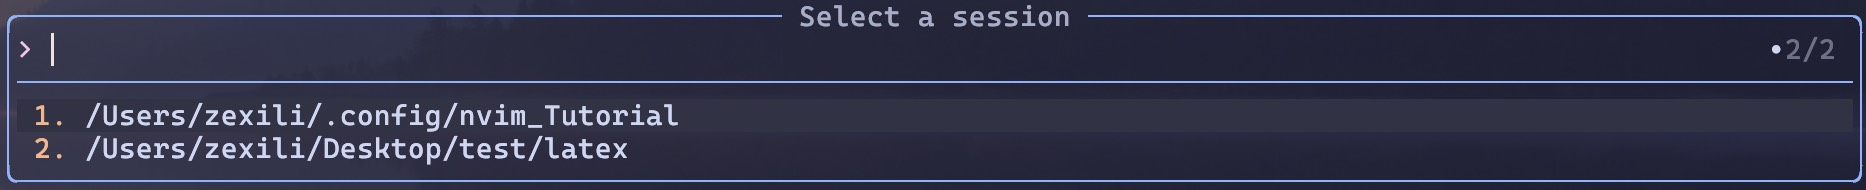
\includegraphics[width=0.8\linewidth]{./Figures/Autosession_Finish_1.jpg}
      \end{figure}
    \item 会话删除
      \begin{figure}[H]
        \centering
        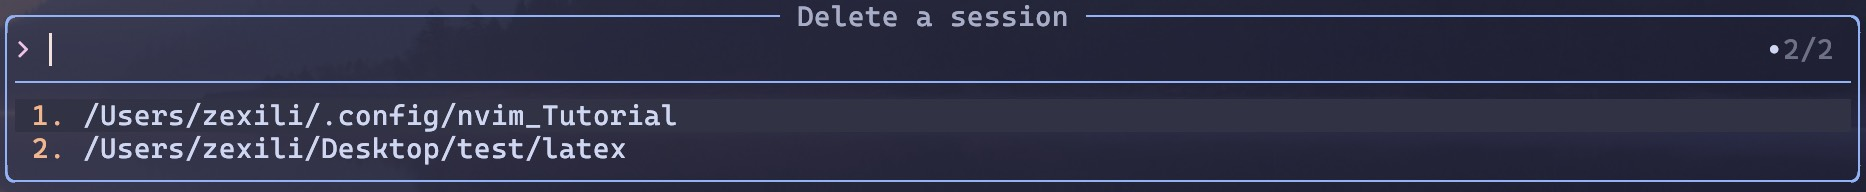
\includegraphics[width=0.8\linewidth]{./Figures/Autosession_Finish_2.jpg}
      \end{figure}
  \end{itemize}
  配置文件:\lstinline[language={},style=path]{\~/.config/nvim/lua/plugins/session.lua}
\end{frame}

\subsection{yazi.nvim: nvim中的yazi文件浏览器集成}
\begin{frame}{\link{yazi.nvim}{https://github.com/mikavilpas/yazi.nvim}: nvim中的yazi文件浏览器集成}
  \begin{figure}[H]
    \centering
    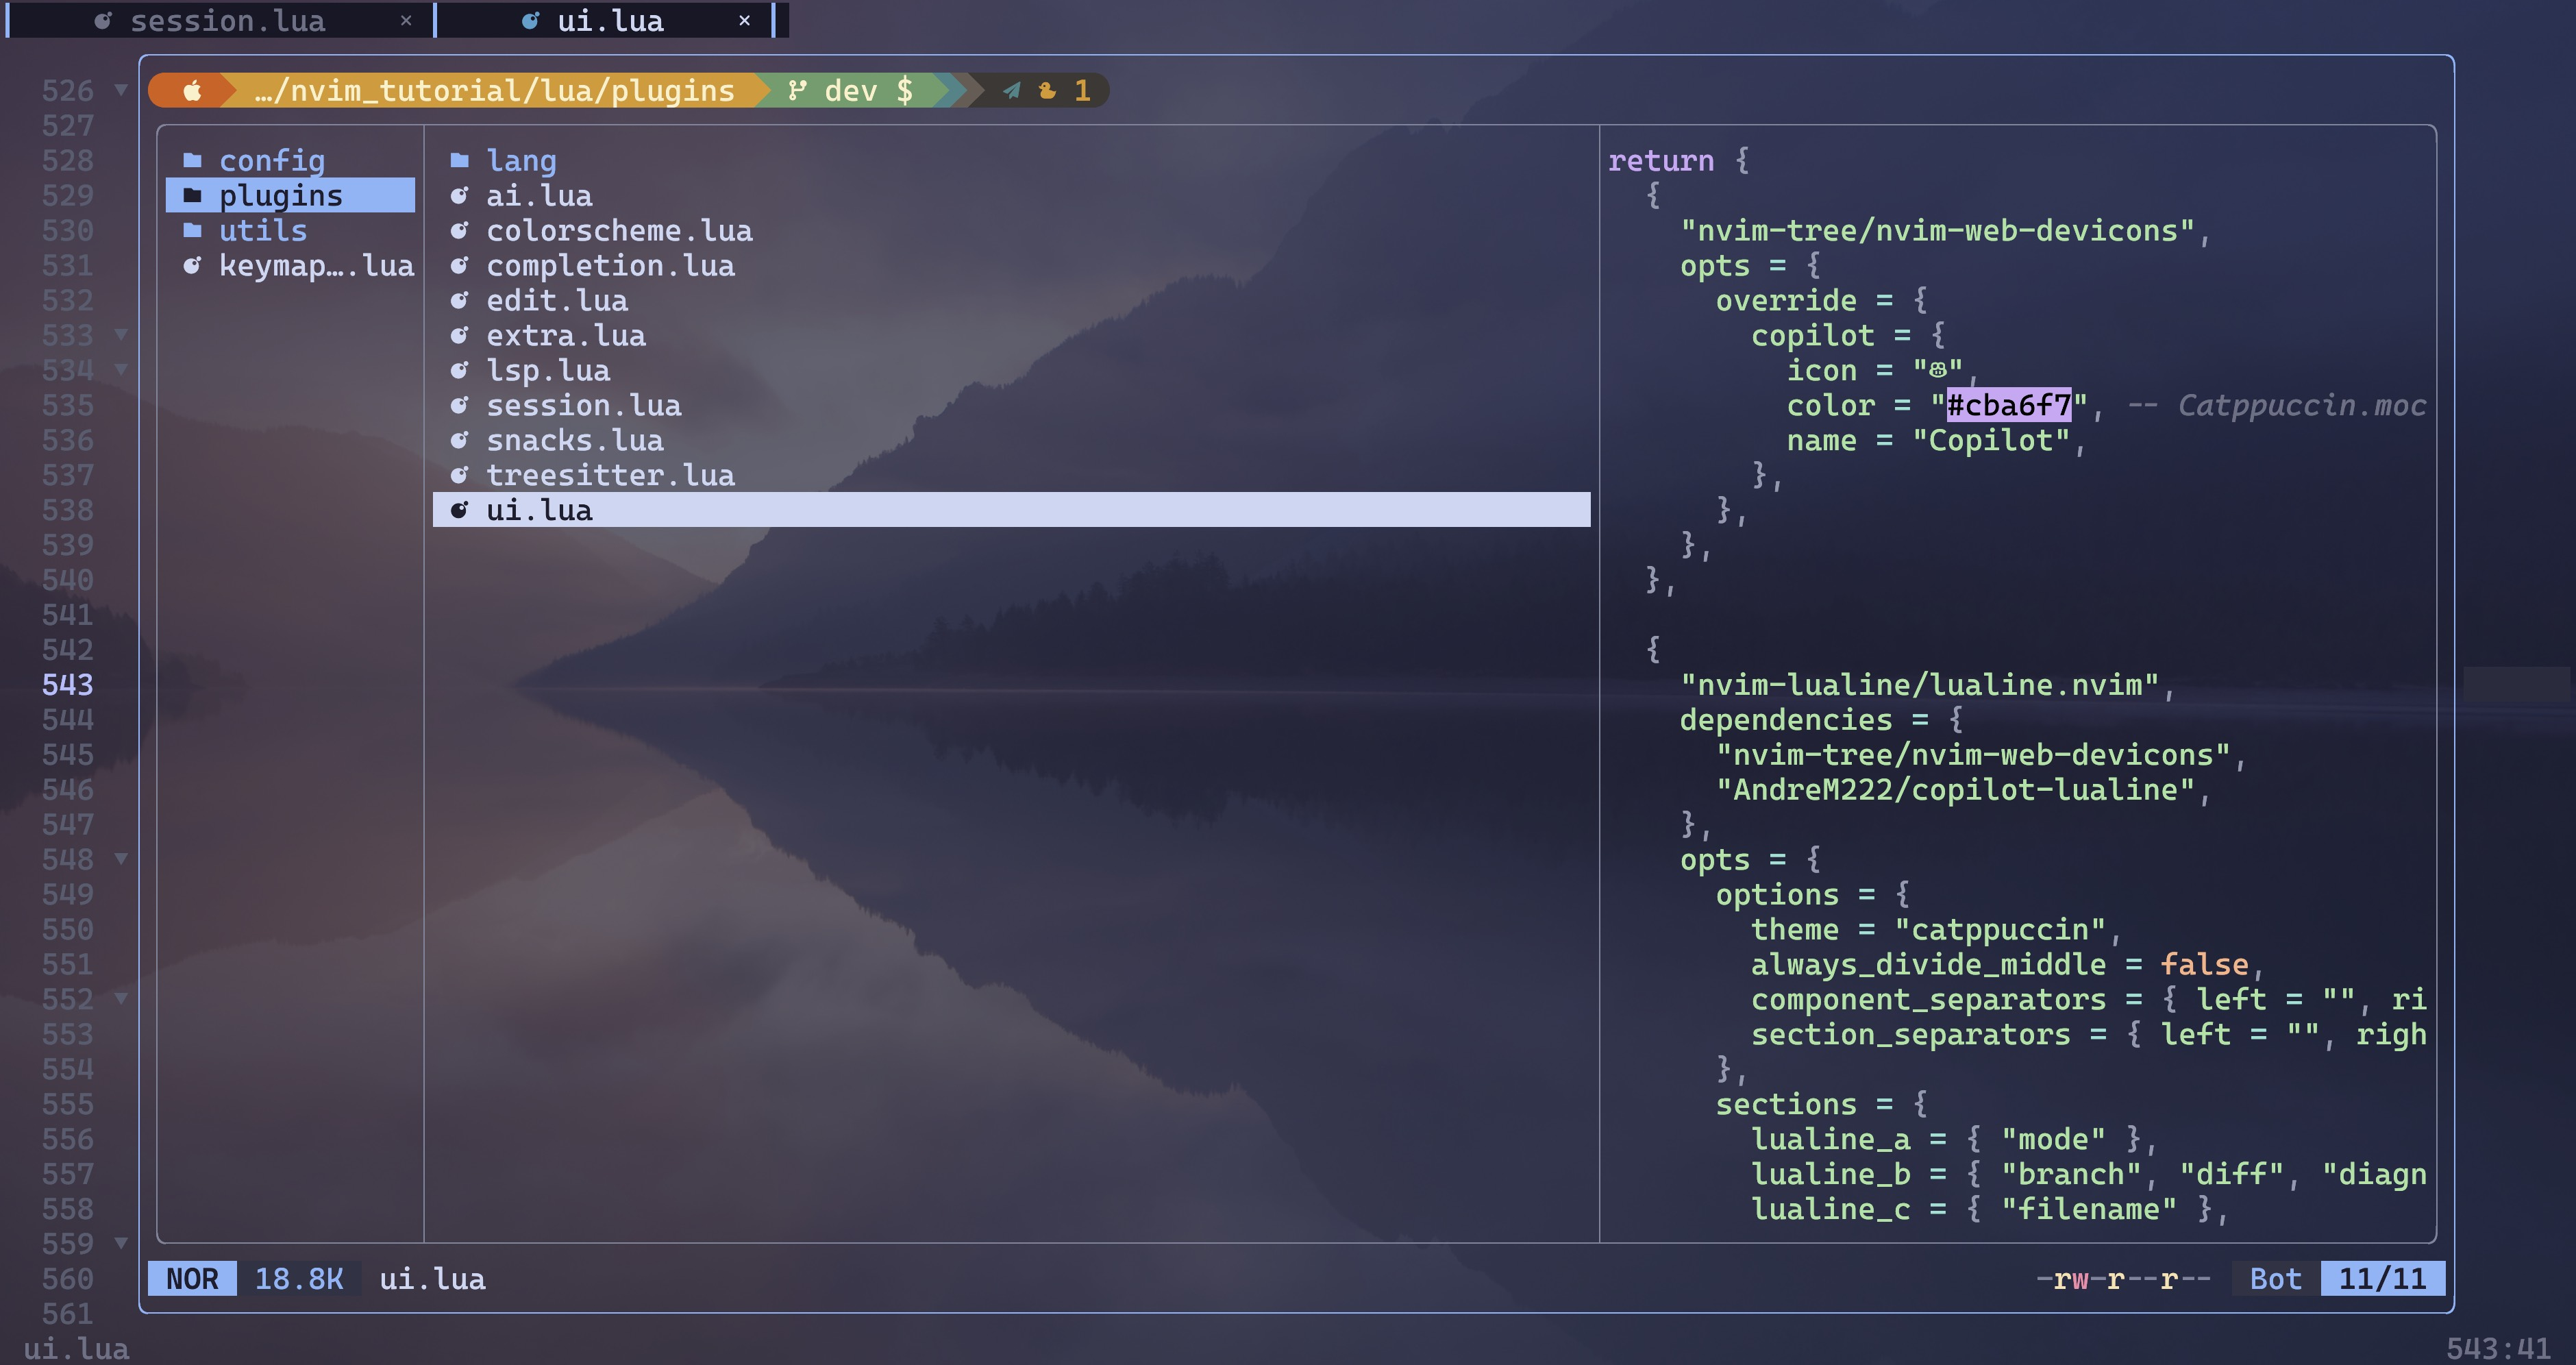
\includegraphics[width=0.65\linewidth]{./Figures/Yazi_Finish.jpg}
  \end{figure}
  配置文件:\lstinline[language={},style=path]{\~/.config/nvim/lua/plugins/ui.lua}
\end{frame}

\subsection{vim-startuptime: nvim启动时间测试}
\begin{frame}{\link{vim-startuptime}{https://github.com/dstein64/vim-startuptime}: nvim启动时间测试}
  \begin{figure}[H]
    \centering
    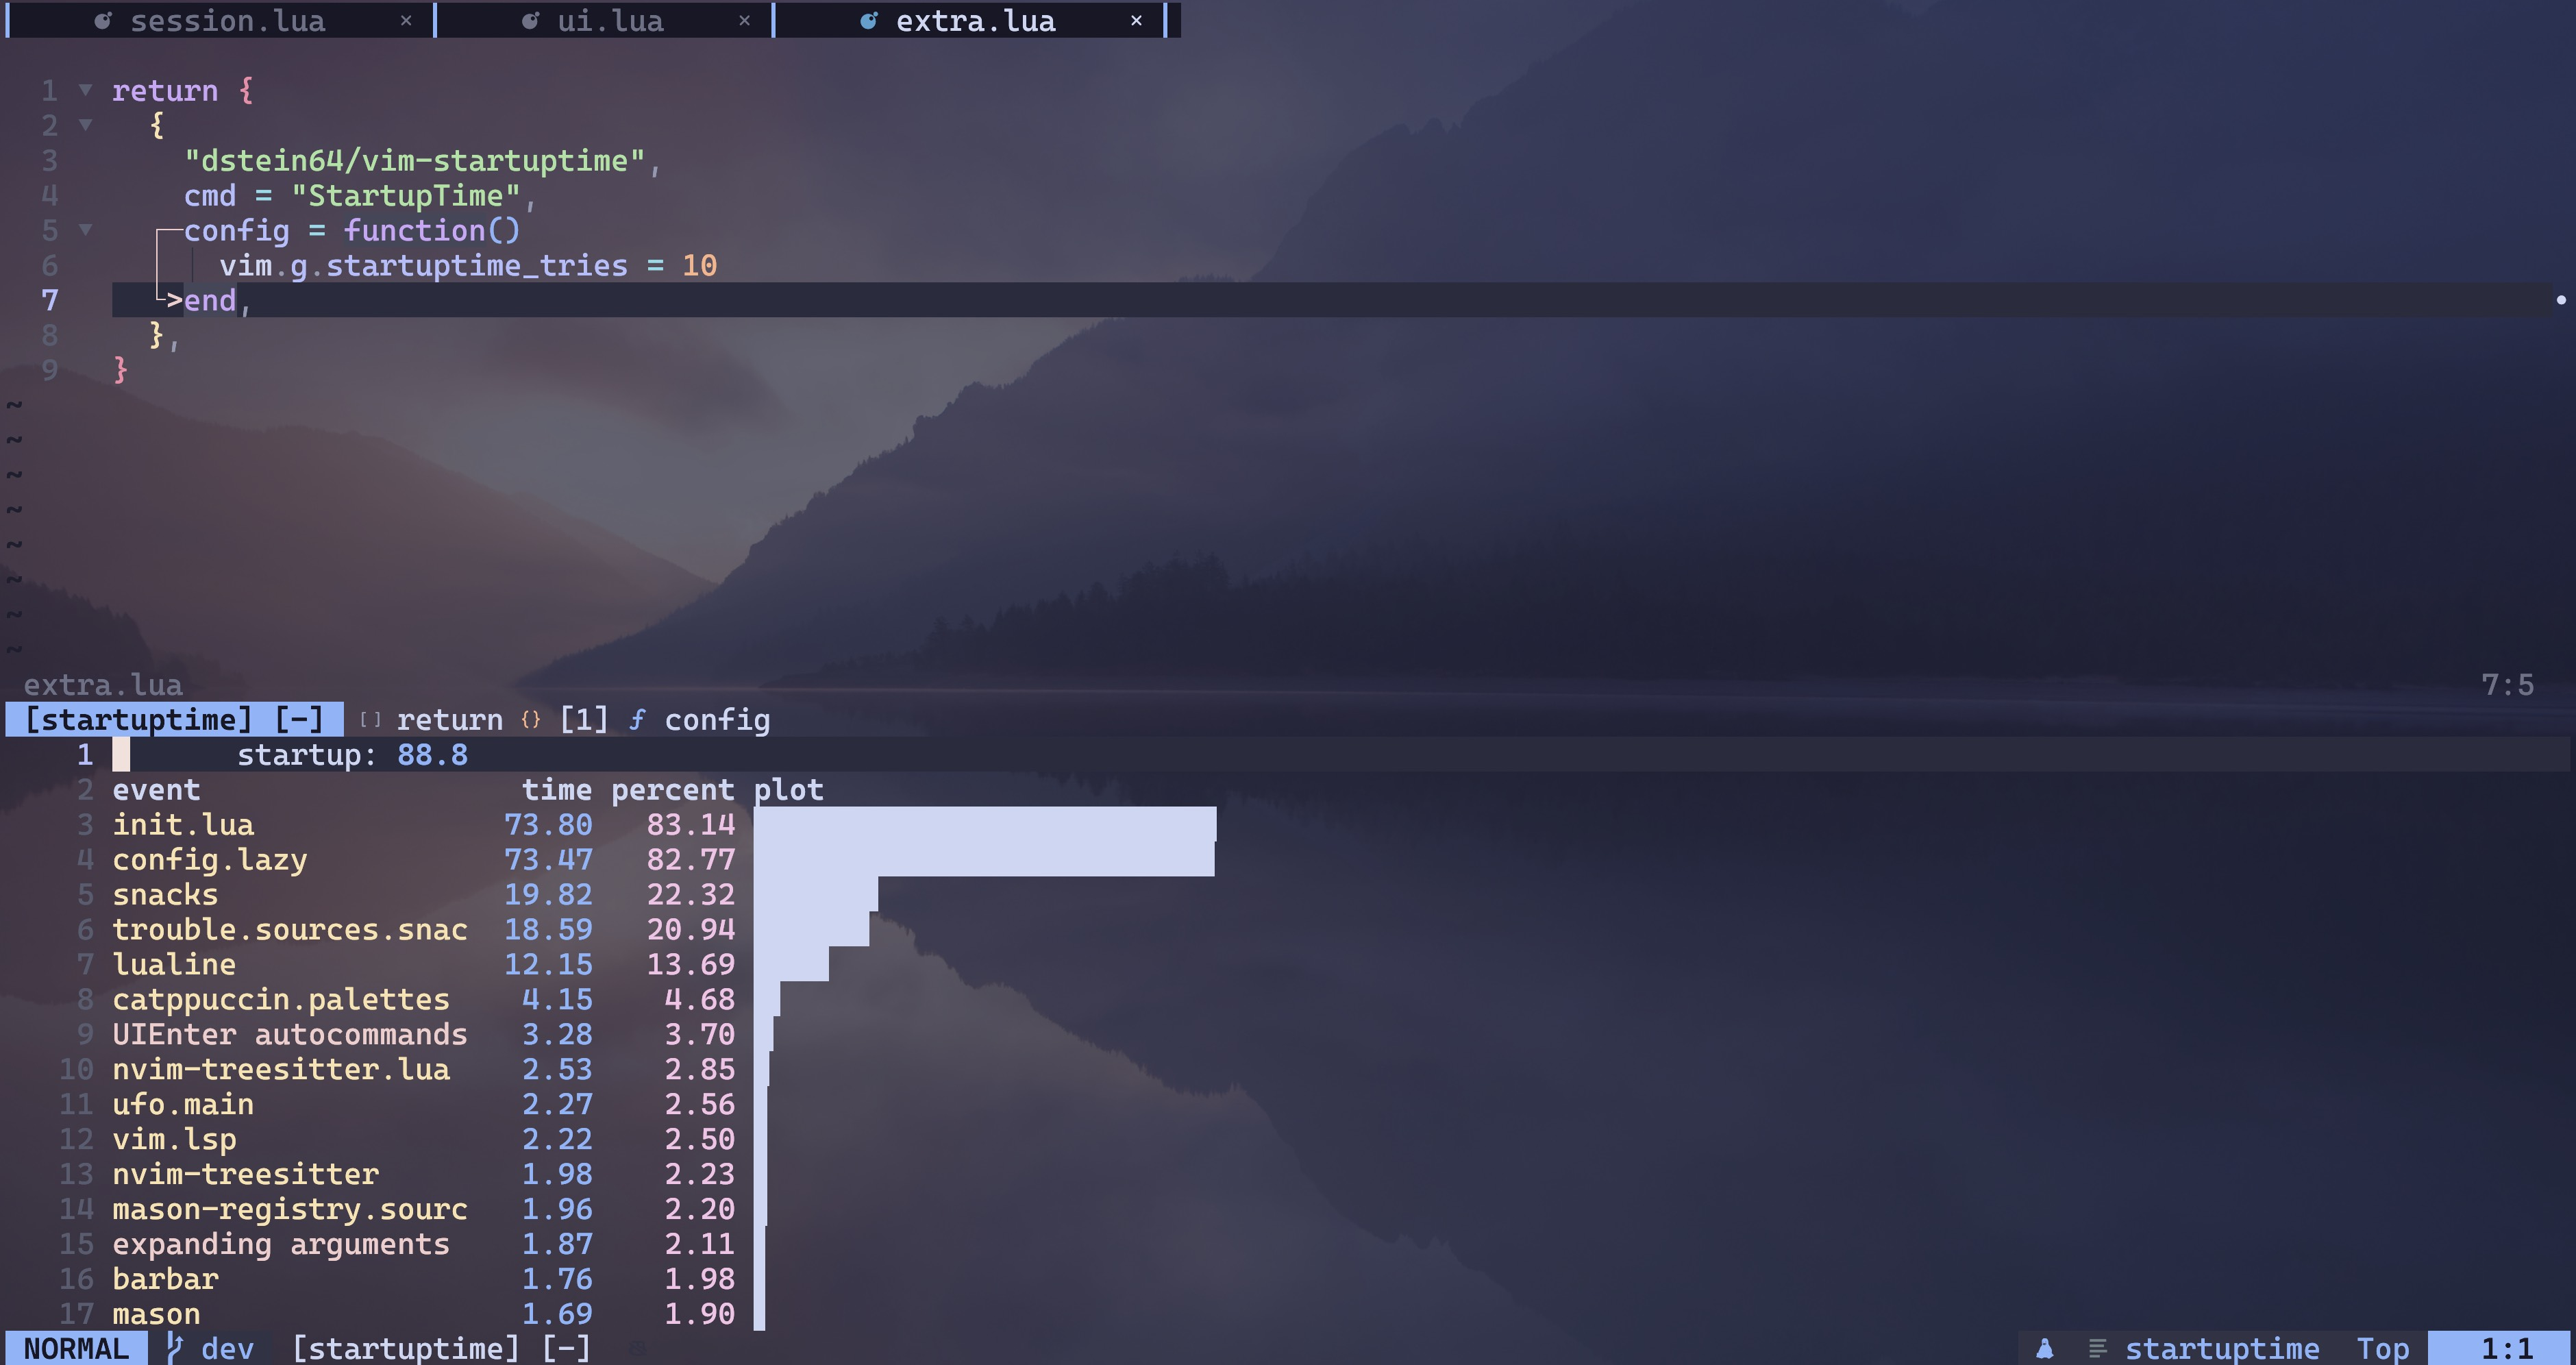
\includegraphics[width=0.65\linewidth]{./Figures/StartupTime_Finish.jpg}
  \end{figure}
  配置文件:\lstinline[language={},style=path]{\~/.config/nvim/lua/plugins/extra.lua}
\end{frame}

\begin{frame}
  \begin{itemize}
    \item 感谢:
      \begin{itemize}
        \item \link{Catppuccin}{https://catppuccin.com/} 
\includegraphics[height=10pt]{./Figures/Catppuccin_logo.png}
        \item \link{Catppuccin for beamer}{https://github.com/atticus-sullivan/beamercolortheme}
      \end{itemize}
      \vspace{0.5cm}
    \item 本教程的全部材料可以在我的Github上找到
      \begin{itemize}
        \item Slides: \url{https://github.com/Jacky-Lzx/nvim.tutorial.slides}
        \item Config: \url{https://github.com/Jacky-Lzx/nvim.tutorial.config}
      \end{itemize}
  \end{itemize}
\end{frame}

\end{document}
